\chapter{Extending the systems beyond \zwave}
\label{extensions}

\section{IP-Cameras}

IP cameras transmit a video stream that can usually be accessed having dedicated mobile 
apps. Under certain circumstances it is possible to have the very same video stream in 
parallel within the \zwshui.
All \zway user interfaces (Web Browser and native apps for IOS and Android) are based on 
off-the-shelf HTML rendering engines supporting standard video and image formats. To 
display the video stream of a certain camera this stream must comply to commonly used 
public standards, such as \textbf{MJPEG}.

Certain cameras however use \textbf{proprietary video encoding} that can only be decoded 
by special native mobile apps of the manufacturers. These cameras can’t be supported by \zway.

\subsection{How to find out if a camera is supported by \zway?}

\begin{enumerate}
\item Check the manual if MJPEG is mentioned as encoding method for the video stream.
\item Check if there is a way to access the video stream using a standard web browser 
such as Google Chrome or Microsoft Internet Explorer.
\end{enumerate}

\subsection{How to prepare for integration?}

To integrate a camera into \zway, this camera needs to be setup first following the 
guidelines given in the manufacturers manual. As a result, there must be

\begin{itemize}
\item A login name (examples are “admin” or “user”)
\item A password for access (this usually needs to be setup
\item The IP address of the camera
\end{itemize}

\subsection{How to find the IP address of the camera?}

Most IP networks in private homes and offices assign IP devices a new IP address using 
the DHCP protocol. The router holds a list of IP addresses and will arbitrarily choose 
one address from the list to the new IP device. Even after a reboot this address will 
remain the same. If the setup process mentioned above does not reveal the IP address 
there are two common ways:
\begin{itemize}
\item Log into your IP routers user interface. Usually this interface will display
 all IP addresses assigned together with a name and/or type of the device.
\item Use an IP address scanner on your PC or notebook that will tell you all IP 
devices active in a network plus the type of IP device they ae assigned to. A valuable 
tool for this is called ``Angry IP Scanner’’ available for all PC platforms such as
 MAC OSX, Linux or Windows. It requires a Java Virtual Machine (JVM).
\end{itemize}

\subsection{How to integrate the camera into \zway?}


\begin{figure}
\begin{center}
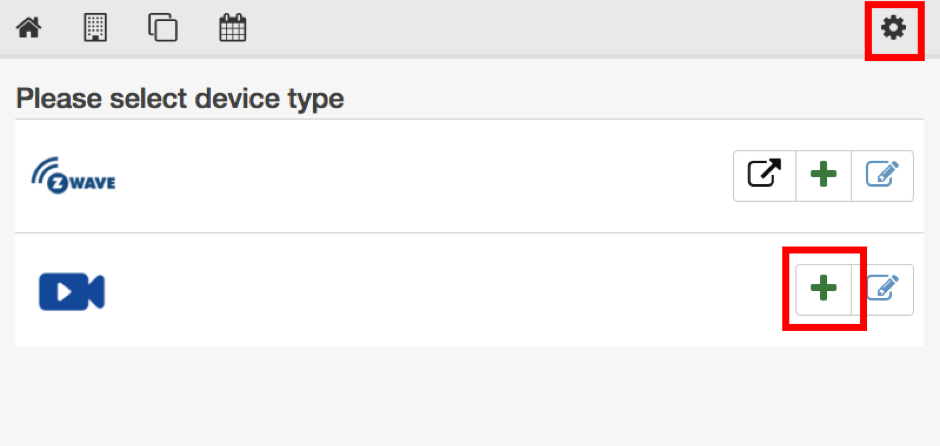
\includegraphics[width=0.7\textwidth]{pngs/cap9/camera1.png}
\caption{Inclusion of predefined cameras}
\label{camera1}
\end{center}
\end{figure}

The \zwshui allows adding new devices. Log into the user interface of \zway, 
click on the setup menu (icon on the upper right side) and click on menu item 
\keystroke{Add New Device}. You see the dialog as shown in Figure \ref{camera1}. Now 
choose the IP camera symbol line and click \keystroke{+}.

\begin{figure}
\begin{center}
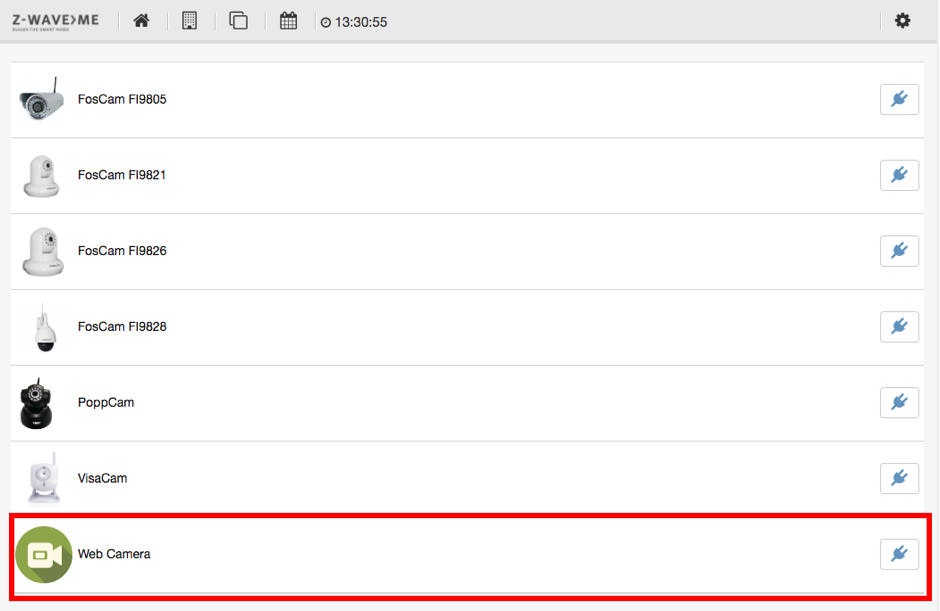
\includegraphics[width=0.7\textwidth]{pngs/cap9/camera2.png}
\caption{Generic camera module}
\label{camera2}
\end{center}
\end{figure}

Now you will find a list of IP camera types plus one generic IP camera option 
called \app{Web Camera}. This dialog is shown in Figure \ref{camera2}.

If you are lucky, the name of your camera is already on the list. If not, you can 
check in the app store if there is a new support app available for your camera type. 
Go to \menu{Setup > App > Online Apps} and filter for \app{Video Surveillance.} 
Figure \ref{camera3} shows the app store with camera filter.

\begin{figure}
\begin{center}
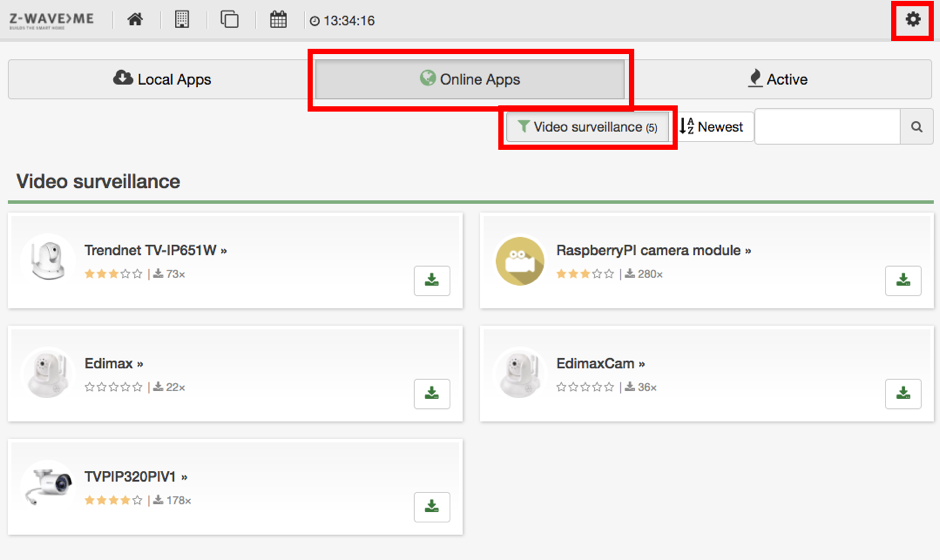
\includegraphics[width=0.7\textwidth]{pngs/cap9/camera3.png}
\caption{More camera support in App Store}
\label{camera3}
\end{center}
\end{figure}

If you find your camera type, just install the app and redo the steps above. Now you will 
find the new camera in the list to choose from.

Once you click on the camera of your choice there will be a setup wizard asking you as a 
minimum for the IP address of your camera, the login name, and the password. Therefore, 
you need this set of data from the setup process of your device.

\subsection{How to support a camera not on the list yet?}

If your camera type is neither on the list of preset cameras nor there is a new app in 
the online app store there is still a very good chance to get your camera integrated. 
However now there is more work needed to find the right commands controlling your camera. 
In this case, you will need to choose the generic camera type ``Web camera,’’ which requires 
the same set of information (IP address, login, password) but more than that.

\begin{figure}
\begin{center}
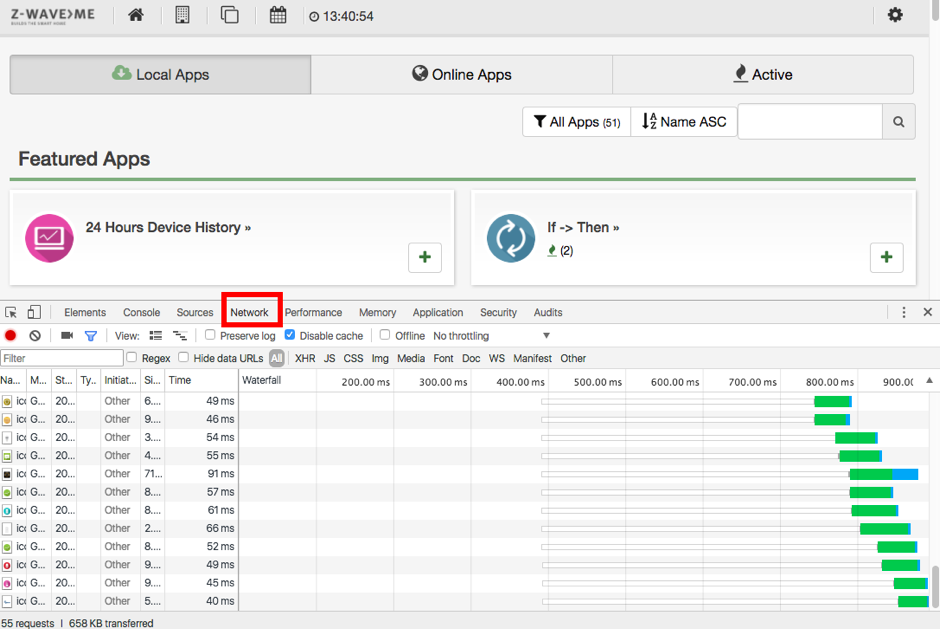
\includegraphics[width=0.7\textwidth]{pngs/cap9/camera4.png}
\caption{Web browser debug interface}
\label{camera4}
\end{center}
\end{figure}

{\em Note: This work requires some basic understanding of web pages, IP, and URLs. The 
generic web camera allows defining the URL to the video stream and---if the camera has 
these capabilities---links to tilt, turn, night vision control, etc.}

To find these URLs, you need to log into your camera using a generic web browser. We 
strongly recommend using Google Chrome because of the debugging capabilities. The 
following explanation assumes the Chrome browser, but other browser will have similar functions.

\begin{enumerate}
\item Open the JavaScript Debug console. You find this option on the browsers menu under
\menu{View > Developer}. Figure \ref{camera4} shows the web browser with debugger active.
\item Once the debugger is open pick the menu item \menu{network} of the debugger (see image below”
\item Now you use the cameras web interface for accessing the image/stream, tilting, moving, 
etc. Whenever you do this the URL needed will be sent from the web interface to the camera 
and becomes visible in the debugger. Take these URLs and copy them into the setup 
interface of \app{Web Camera}. The camera control in \zwave will call the same URL for 
control.
\end{enumerate}

\section {EnOcean devices}

EnOcean is another wireless communication technology optimized for very low power consumption.

\zway has implemented support for EnOcean devices but limits its function to sensors and 
wall switches because of their battery-free and therefore maintenance-free design. Compared 
to \zwave, EnOcean is a quite simple protocol. There is no such thing like network 
inclusion or routing---every EnOcean device just sends out a specific datagram that 
includes a unique device id and the data (sensor values, switch status) of the specific 
function of the device. The encoding of these data is defined in so-called profiles. These 
profiles are identified by a three-byte value but they are not transmitted wirelessly. 
Hence the user must decide from his product knowledge what profile a certain device is 
using. The EnOcean receiver will use this information to decode the datagram and use the 
data. (This means that a wrong decision about the profile of a EnOcean device will lead 
to severe malfunctions of the system).


Every EnOcean receiver in proximity will always receive every datagram sent by a transmitter. 
This leads to two basic management functions of the EnOcean module:
\begin{enumerate}
\item select the right products (by their unique 4 Byte ID) to use---and ignore all others
\item define the correct profile by selecting the right product
\end{enumerate}


\begin{figure}
\begin{center}
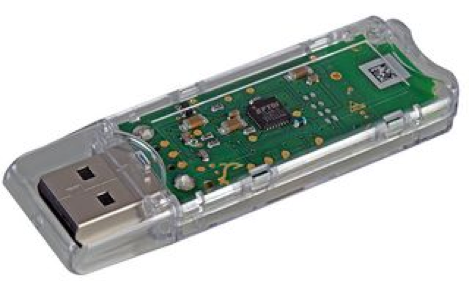
\includegraphics[width=0.4\textwidth]{pngs/cap9/enocean1.png}
\caption{Popp EnOcean USB Stick}
\label{enocean1}
\end{center}
\end{figure}

To work with EnOcean devices, an EnOcean USB Stick is required. Please use the Popp 
EnOcean Stick (POPE12204) as shown in Figure \ref{enocean1} and plug it into the USB 
port\footnote{Other EnOcean sticks may work as well, but the correct function is not 
supported and they may stop working after \zway firmware updates.}.

Next, the EnOcean app must be installed from the app store and configured as 
shown in Figure \ref{enocean2}.

\begin{figure}
\begin{center}
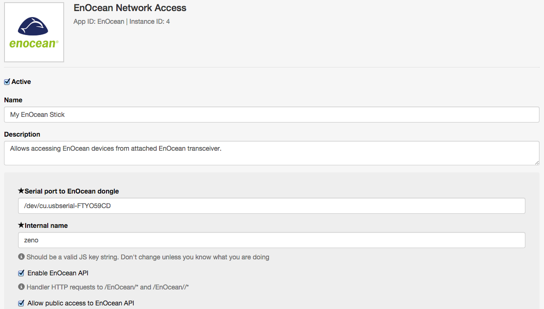
\includegraphics[width=0.7\textwidth]{pngs/cap9/enocean2.png}
\caption{EnOcean App configuration}
\label{enocean2}
\end{center}
\end{figure}

Make sure to pick the right device name of the EnOcean USB Stick connected to your 
hardware. For Raspberry Pi-based platforms this is always \cmdline{/dev/USB0} but for other 
platforms this may be different. The internal name, ``zeno,’’ can be arbitrarily chosen. 
In case more than one EnOcean stick is operated this name needs to be unique.

\begin{figure}
\begin{center}
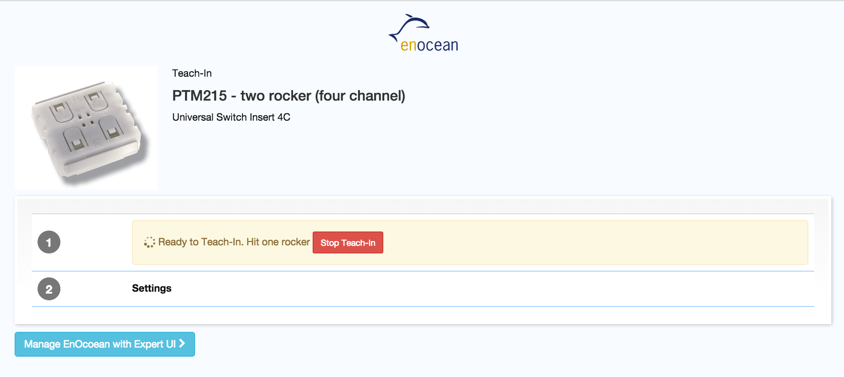
\includegraphics[width=0.7\textwidth]{pngs/cap9/enocean3.png}
\caption{EnOcean Teach In}
\label{enocean3}
\end{center}
\end{figure}

Now it is possible to ``teach-in’’ new products using the user interfaces ``Device’’ 
section \menu{Configuration > Device > EnOcean}.

As described above the first step is to select the right product. A list of manufacturers 
with their products are given to select from. Please note that the EnOcean module may 
support many more devices from other manufacturers as long as they have the same profile. 
A good example for this is a door window sensor (profile name D5-00-01). Multiple 
manufacturers off door-window sensors, some even in the same enclosure but some in 
slightly changed enclosure. Their EnOcean wireless capability is however similar.

You may find the profile name on the label of the unknown device or documented in the 
device specification of the manufacturer.

\textbf{Please not that without proper knowledge of the device and its profile it is 
impossible to operate the device!}

After selecting the right device, the user interface asks for the teach-in process 
as shown in Figure \ref{enocean3}. During this process, the new device must send 
out one datagram containing the unique ID. The user interface will give some 
hints how to generate such a datagram.

\begin{figure}
\begin{center}
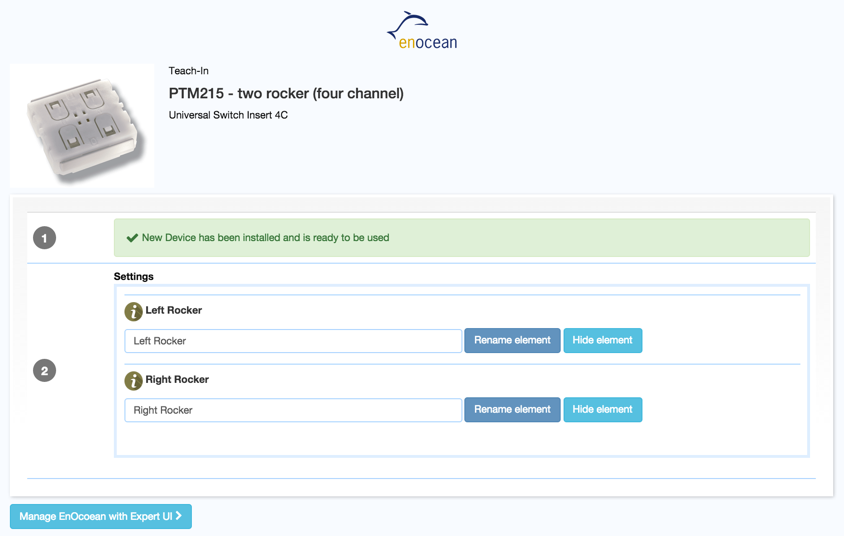
\includegraphics[width=0.7\textwidth]{pngs/cap9/enocean4.png}
\caption{EnOcean Device Configuration after Teach-In}
\label{enocean4}
\end{center}
\end{figure}

Once this datagram was received, the EnOcean module will generate virtual devices 
according to the profile selected. You can change the names of the elements to be 
generated. Figure \ref{enocean4} shows this dialog.

Finally, as shown in Figure \ref{enocean5} one or multiple elements will appear in 
the elements view. One example of the wall controller device shows Figure \ref{enocean6}.

\begin{figure}
\begin{center}
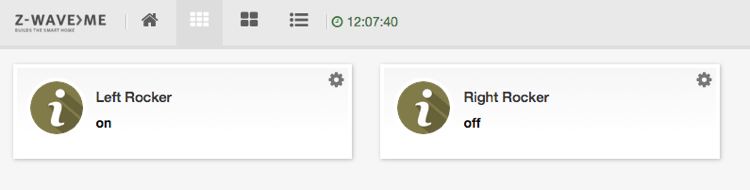
\includegraphics[width=0.7\textwidth]{pngs/cap9/enocean5.png}
\caption{EnOcean Device Elements}
\label{enocean5}
\end{center}
\end{figure}

The menu option \menu{Devices} also offers a special interface to manage EnOcean devices as 
shown in Figure \ref{enocean6}. This dialog offers a list of all known EnOcean devices 
with an option to change the profile.
Furthermore, it is possible to manually select one of the valid profiles of EnOcean for
 a device not known to the standard user interface. Please note that profiles not known 
 to the standard UI are also not supported by the standard user interface and will not 
 leads to creating new UI elements. However, the device is still created in the API 
 and can be used by third-party software.

\begin{figure}
\begin{center}
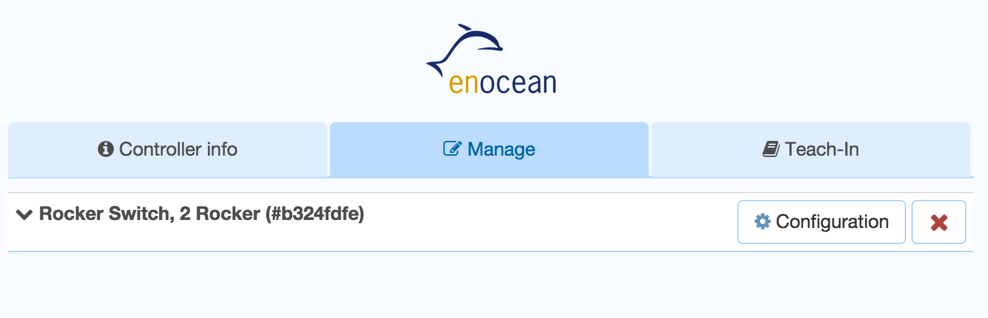
\includegraphics[width=0.7\textwidth]{pngs/cap9/enocean6.png}
\caption{EnOcean Device Management}
\label{enocean6}
\end{center}
\end{figure}

For a list of all supported EnOcean devices, please refer to Annex \ref{annexenocean}.
Experienced Users and programmers may extend this list by adding their own profiles to \zway.
Chapter \ref{addenocean} describes how to do this.


\section {Other IP/Internet-based services}

\zway can work with external IP-based systems. Please refer to the app store description 
for more information about how to integrate third-party IP-based devices. Please refer 
to Chapter \ref{apps} for details.

